Es gibt verschiedene Möglichkeiten das magnetische Moment zu messen. In diesem Versuch wird die Hochfrequenz-Methode verwendet, die im folgenden Kapitel erklärt wird. Danach wird der gesamte Aufbau des Experiments und die Durchführung der Messung beschrieben.
\todo{Ich habe hier den Satz darüber was genau bei der Resonanz passiert eingefügt, sonst verstehe ich das in zwei Wochen schon nicht mehr :P}
\subsection{Hochfrequenz-Methode}
Die Hochfrequenz-Methode basiert auf der Aufspaltung der Energieniveaus, wenn ein magnetisches Moment in ein Magnetfeld gebracht wird. Für Elektronen (Spin~$\frac{1}{2}$) entstehen zwei Zustände, wobei der Zustand mit niedrigerer Energie~$E_0$ bei Raumtemperatur im thermodynamischen Gleichgewicht stärker besetzt ist als der Zustand mit der höheren Energie~$E_1$. Elektronen können durch Energiezufuhr von Zustand $E_0$ in $E_1$ gebracht werden. Die Energie wird durch ein elektromagnetisches Feld bereitgestellt. Damit ein Übergang möglich ist, müssen das Magnetfeld und die Frequenz~$\nu$ des elektromagnetischen Feldes aufeinander so abgestimmt sein, dass die Resonanzbedingung 
\begin{equation}\label{eq:DeltaE}
	\Delta E = \textrm{h} \nu = g \mu_\textrm{B} B
\end{equation}
erfüllt ist (siehe Abb. \ref{fig:elektron}). Nur dann klappen die Spins um. \\
Für Magnetfelder mit einer Stärke von einigen \si{\milli\tesla} liegt die Resonanzfrequenz im hochfrequenten Bereich mit ungefähr \SI{100}{\mega\hertz} und für Felder mit der Magnetfeldstärke einiger \si{\tesla} im Mikrowellen Bereich.
\\
\begin{figure}[h!]
	\centering
	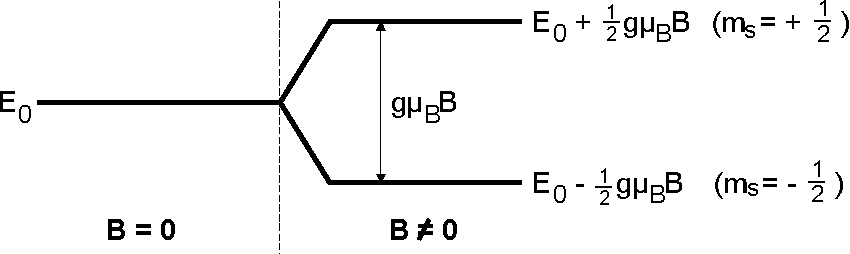
\includegraphics[width=0.6\textwidth]{Anleitung_Abb6.pdf}
	\caption[Energieniveaus]{Energieniveaus des Elektrons \cite{V28}}
	\label{fig:elektron}
\end{figure}


\clearpage
\subsection{Aufbau des Versuchs}
Die technische Umsetzung der Hochfrequenzmethode ist in Abb. \ref{fig:aufbau} dargestellt. Die Probe (Diphenylpikrylhydrazyl) befindet sich in einer Hochfrequenz-Spule, die ein elektromagnetisches Feld erzeugt. Der quarzstabile Oszillator gibt dabei die Frequenz vor. In Kombination mit der elektrischen Brücke werden hohe Genauigkeiten für die Frequenz des Feldes erreicht. Die Frequenz ist für die einzelnen Messungen konstant. Die Stärke des Magnetfeldes ist hingegen variabel. Das Magnetfeld wird durch zwei Helmholtz-Spulen erzeugt und lässt sich über den Rampengenerator mit Gleichstrom steuern. Ist Bedingung \eqref{eq:DeltaE} aus dem vorangegangenen Abschnitt erfüllt, klappen die Spins um und erhöhen damit die Induktivität der Spule, sodass die Brücke verstimmt wird und eine Spannung am Ausgang der Brücke gemessen werden kann. \\
Am X-Y-Schreiber trifft zum einen die Stromstärke, die das Magnetfeld erzeugt, ein. Sie wird auf die X-Achse des Schreibers gelegt. Zum anderen wird das Signal aus der Brücke an die Y-Achse angelegt. Dieses Signal zeigt die Resonanz der Probe. Es ist sehr schwach und wird mit einem Überlagerungsempfänger verstärkt.

 \begin{figure}[h!]
	\centering
	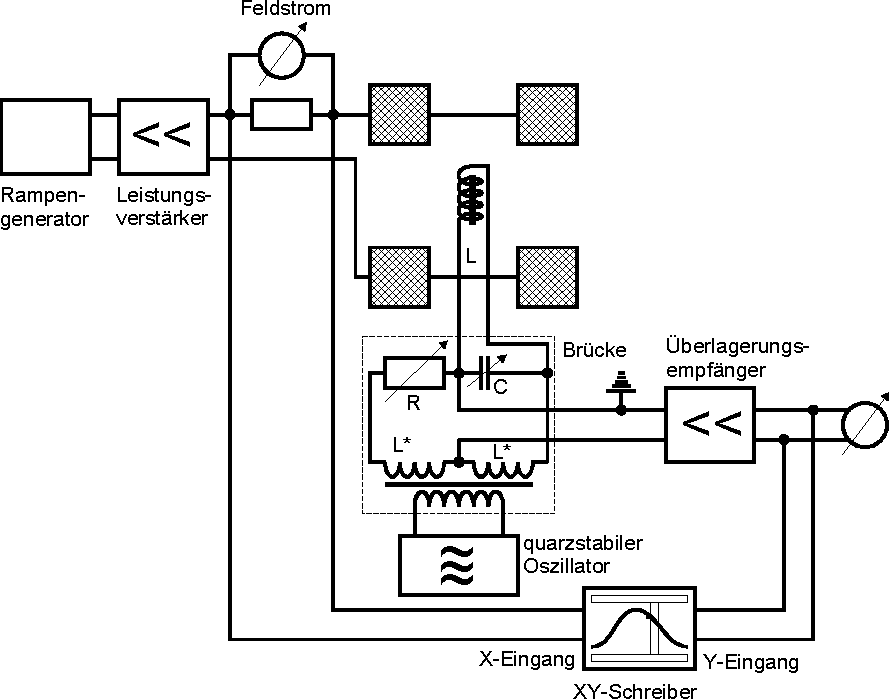
\includegraphics[width=0.8\textwidth]{Anleitung_Abb8.pdf}
	\caption[Versuchsaufbau]{Versuchsaufbau für die Durchführung der Hochfrequenz-Methode \cite{V28}}
	\label{fig:aufbau}
\end{figure}
\clearpage
Der Überlagerungsverstärker (siehe Abb. \ref{fig:verstaerker}) funktioniert wie folgt: Das Eingangssignal mit der Frequenz~$\nu_e$ wird so weit es geht verstärkt und nicht gewünschte Frequenzen  heraus gefiltert. Dann wird das Signal mit einem zweiten überlagert. Die Frequenz des zweiten Signal~$\nu_\textrm{Osz}$ ist gerade so gewählt, dass eine Schwebung mit der Zwischenfrequenz $\nu_\textrm{ZF} = \nu_e - \nu_\textrm{Osz}$ auftritt. Die Zwischenfrequenz liegt in einem Bereich, dass sie leicht verstärkt und gleichgerichtet werden kann. So gelangt das Signal zum X-Y-Schreiber.


\begin{figure}[h!]
	\centering
	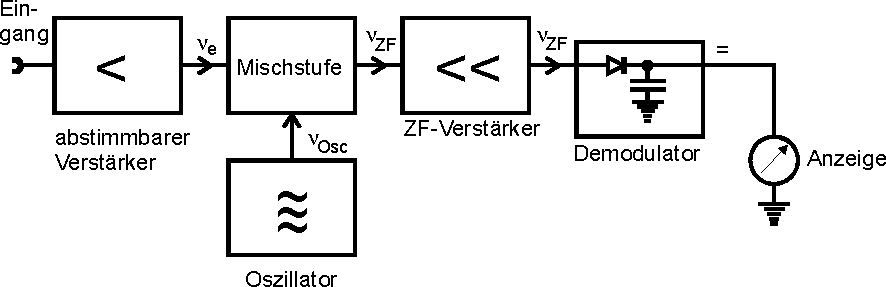
\includegraphics[width=0.8\textwidth]{Anleitung_Abb9.pdf}
	\caption[Blockschlatbild eines Überlagerungsempfängers]{Blockschlatbild eines Überlagerungsempfängers \cite{V28}}
	\label{fig:verstaerker}
\end{figure}




\clearpage

\subsection{Messung}
Es werden für fünf verschiedene Frequenzen die Resonanzen gemessen, indem die Stärke des Magnetfeldes variiert wird. Um optimale Messergebnisse zu erzielen, müssen für jede Messung die Geräte aufeinander abgestimmt werden. Wichtig ist, dass beim Einstellen immer globale Extrema gesucht werden.

\begin{enumerate}
	
\item{Der gewünschte \textbf{Frequenzbereich} (10, 15, 20, 24.44 oder \si{30}{\mega\hertz}) wird ausgewählt und die Geräte darauf eingestellt.}

\item{Die Frequenz des \textbf{Überlagerungssignals} wird so eingestellt, dass sie zirka um \si{552}{\kilo\hertz} von der Eingangsfrequenz abweicht. Das Ausgangssignal soll so groß wie möglich sein.}

\item{Die \textbf{Brückenschlatung} wird zunächst über die Einstellung $C_\textrm{grob}$ und dann über $C_\textrm{fein}$ und $R_\textrm{Abgleich}$ so angepasst, dass das Ausgangssignal minimiert wird. Der Signalverstärker muss so niedrig wie möglich eingestellt sein. Dazu wird bei einem  Ausgangssignal von knapp über \si{0,065}{\volt} der Verstärker so variiert, dass die Spannung wieder ein Maximum einnimmt. Minimiert wird dann wieder mit Hilfe des Einstellens von $C_\textrm{fein}$ und $R_{\textrm{Abgleich}}$.}

\item{Um die charakteristische \textbf{Lorentz-Kurve} (siehe Abb. \ref{fig:kurve}) zu erhalten, muss das Ausgangssignal durch die Veränderung von $R_\textrm{Abgleich}$ bis auf ungefähr  \si{0,2}{\volt} erhöht werden.}

\item{Der \textbf{X-Y-Schreiber} wird so eingestellt, dass er die Kurve komplett aufnimmt.}
\item{Der X-Y-Schreiber wird für jede Messung einzeln kalibriert, indem für fünf Werte in X-Richtung die Stromstärke notiert wird.\label{Schritt6}}
\end{enumerate}
Die Messung wird jeweils einmal parallel und einmal antiparallel zum Erdmagnetfeld durchgeführt und in eine Grafik gezeichnet.

\begin{figure}[h!]
	\centering
	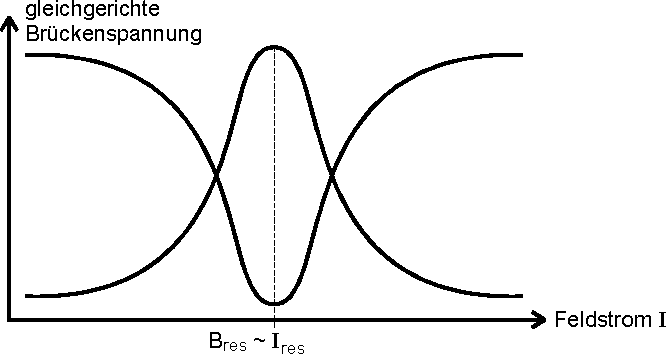
\includegraphics[width=0.6\textwidth]{Anleitung_Abb10.pdf}
	\caption[Resonanzkurve]{Gesuchte Resonanzkurve (Lorentz-Kurve) \cite{V28}}
	\label{fig:kurve}
\end{figure}
